
\de{ĐỀ THI HỌC KỲ I NĂM HỌC 2022-2023}{Sở Giáo Dục Bắc Giang}
\begin{center}
	\textbf{PHẦN 1 - TRẮC NGHIỆM}
\end{center}
\Opensolutionfile{ans}[ans/ans]
%Câu 1...........................
\begin{ex}%[0T4B1-2]%[Dự án đề kiểm tra HKII NH22-23- Tên GV]%[Tên Trường]
Tính giá trị của biểu thức $P=\sin 75^\circ +\sin 55^\circ-\cos 15^\circ+\cos 145^\circ+\cos 180^\circ$.
	\choice
	{$P=0$}
	{\True $P=-1$}
	{$P=1$}
	{$P=2$}
	\loigiai{$P=\sin 75^\circ +\sin 55^\circ-\cos 15^\circ+\cos 145^\circ+\cos 180^\circ=-1$.
		
	}
\end{ex}
\begin{ex}%[0T2B1-2]%[Dự án đề kiểm tra HKII NH22-23- Phạm Văn Long]%[SGD Bắc Giang]
	Phần không gạch (kể cả đường thẳng $\Delta$) trong hình bên dưới biểu diễn miền nghiệm của bất phương trình nào trong các bất phương trình sau?
	\begin{center}
		\begin{tikzpicture}[scale=0.7, line join=round, line cap=round, >=stealth]
			\tikzset{every node/.style={scale=0.8}}
			\def\xmin{-1}\def\xmax{4}\def\ymin{-1}\def\ymax{3}
			\fill [pattern=north east lines,pattern color=blue!20] plot[smooth,samples=200,domain=\xmin:\xmax](\x,{-2/3*(\x)+2})--(\xmax,\ymax)--(\xmin,\ymax);			
			\draw[->] (\xmin-0.2,0)--(\xmax+0.3,0) node[above] {$x$};
			\draw[->] (0,\ymin-0.2)--(0,\ymax+0.3) node[left] {$y$};
			\draw (0,0) node [below left] {$O$};
			\draw (4,-0.8) node [left] {$\Delta$};
			\foreach \x in {3}\draw (\x,0.1)--(\x,-0.1) node [below] {$\x$};
			\foreach \y in {2}\draw (0.1,\y)--(-0.1,\y) node [above right] {$\y$};
			\clip (\xmin,\ymin) rectangle (\xmax,\ymax);
			\draw[thick,smooth,samples=200,domain=\xmin:\xmax] plot (\x,{-2/3*(\x)+2});
		\end{tikzpicture}
	\end{center}
	\choice
	{\True $2x+3y\le 6$}
	{$2x+3y< 6$}
	{$2x+3y\ge 6$}
	{$2x-3y\le 6$}
	\loigiai{
		Ta thấy đường thẳng $2x+3y=6$ qua hai điểm $(3;0)$ và $(0;2)$, miền nghiệm chứa gốc tọa độ $(0;0)$. Nên miền nghiệm trên là $2x+3y\le 6$.
	}
\end{ex}
\begin{ex}%[0T5Y1-1]%[Dự án đề kiểm tra HKII NH22-23- Phạm Văn Long]%[SGD Bắc Giang]
	 Cho đoạn thẳng $AB$. Gọi $M$ là điểm thuộc đoạn thẳng $AB$ sao cho $AM=\dfrac{3}{4} AB$. Mệnh đề nào dưới đày là đúng?
	\choice
	{\True $\overrightarrow{M A}=-3 \overrightarrow{M B}$}
	{$\overrightarrow{M B}=-3 \overrightarrow{M A}$}
	{$\overrightarrow{M A}=3 \overrightarrow{M B}$}
	{$\overrightarrow{M B}=3 \overrightarrow{M A}$}
	\loigiai{Ta có $M$ thuộc đoạn thẳng $AB$ sao cho $AM=\dfrac{3}{4} AB \Rightarrow \overrightarrow{M A}=-3 \overrightarrow{M B}$.
	}
\end{ex}
\begin{ex}%[0T3B2-1]%[Dự án đề kiểm tra HKII NH22-23- Phạm Văn Long]%[SGD Bắc Giang]
	Biết rằng parabol $y=x^2+bx+c$ có đỉnh là $I(2 ;-1)$. Tính giá trị của biểu thức $b+2c$.
	\choice
	{$-2$}
	{\True $2$}
	{$-1$}
	{$1$}
	\loigiai{Parabol $y=x^2+bx+c$ có đỉnh là $I(2 ;-1)$ suy ra $\heva{&-\dfrac{b}{2}=2\\&2b+c=-5}\Leftrightarrow \heva{&b=-4\\&c=3.}$\\
	Vậy	$b+2c=2$.
	}
\end{ex}
\begin{ex}%[0T5B4-1]%[Dự án đề kiểm tra HKII NH22-23- Phạm Văn Long]%[SGD Bắc Giang]
	Cho tam giác $ABC$ đều cạnh bằng $4$. Tính tích vô hướng $\overrightarrow{AB} \cdot \overrightarrow{BC}$.
	\choice
	{$8$}
	{$-8 \sqrt{3}$}
	{\True $-8$}
	{$-8 \sqrt{3}$}
	\loigiai{
		Ta có $\overrightarrow{AB} \cdot \overrightarrow{BC}=-\overrightarrow{BA} \cdot \overrightarrow{BC}=-4\cdot 4\cdot \cos 60^\circ=-8$.
		
	}
\end{ex}
\begin{ex}%[0T4B2-1] %[Dự án đề kiểm tra HKII NH22-23- Phạm Văn Long]%[SGD Bắc Giang]
	Cho tam giác $ABC$ có $\widehat{A}=120^{\circ}$, $\widehat{B}=15^{\circ}$ và $AB=10 \mathrm{~cm}$. Tính độ dài cạnh $BC$ của tam giác $ABC$.
	\choice
	{$BC=3 \sqrt{6} \mathrm{~cm}$}
	{$BC=20 \sqrt{6} \mathrm{~cm}$}
	{$BC=10 \sqrt{6} \mathrm{~cm}$}
	{\True $BC=5 \sqrt{6} \mathrm{~cm}$}
	\loigiai{
		Áp dụng định lí Sin ta có $\dfrac{BC}{\sin A}=\dfrac{AB}{\sin C}\Rightarrow BC=\dfrac{AB\cdot \sin A}{\sin C}=\dfrac{10\cdot \sin120^\circ}{\sin 45^\circ}=5 \sqrt{6} \mathrm{~cm}$.
		
	}
\end{ex}
\begin{ex}% [0T3B1-5] %[Dự án đề kiểm tra HKII NH22-23- Phạm Văn Long]%[SGD Bắc Giang]
	Hàm số $y=-x^2-2x+3$ đồng biến trên khoảng nào?
	\choice
	{$(-\infty ; 0)$}
	{$(-3 ;+\infty)$}
	{$(-1 ;+\infty)$}
	{\True $(-\infty ;-1)$}
	\loigiai{Hàm số $y=-x^2-2x+3$ đồng biến trên khoảng $(-\infty;-1)$ và $(-1;+\infty)$.
		
	}
\end{ex}
\begin{ex}%[0T3Y2-1]%[Dự án đề kiểm tra HKII NH22-23- Phạm Văn Long]%[SGD Bắc Giang]
	Hàm số nào dưới đây là hàm số bậc hai biến số $x$?
	\choice
	{$y=\dfrac{x^2+1}{x+1}$}
	{$y=\sqrt{3-x^2}$}
	{$y=3-x$}
	{\True $y=-x^2+2x+5$}
	\loigiai{
		Hàm số bậc hai biến số $x$ là $y=-x^2+2x+5$.
		
	}
\end{ex}
\begin{ex}%[0T7B3-1] %[Dự án đề kiểm tra HKII NH22-23- Phạm Văn Long]%[SGD Bắc Giang]
	Số nào đưới đây là nghiệm của phương trình $\sqrt{2x^2+x+3}=\sqrt{x^2+2x+5}$ ?
	\choice
	{$x=-3$}
	{\True $x=2$}
	{$x=-2$}
	{$x=1$}
	\loigiai{
		\allowdisplaybreaks
		\begin{eqnarray*}
		\sqrt{2x^2+x+3}=\sqrt{x^2+2x+5}&\Leftrightarrow& 2x^2+x+3=x^2+2x+5\\
		&\Leftrightarrow& x^2-x-2=0\\
		&\Leftrightarrow&\hoac{&x=-1\\&x=2.}
		\end{eqnarray*}
	}
\end{ex}
\begin{ex}%[0T5B2-1]%[Dự án đề kiểm tra HKII NH22-23- Phạm Văn Long]%[SGD Bắc Giang]
	Trên mặt phẳng cho ba điểm phân biệt $M$, $N$ và $P$. Mệnh đề nào dưới đây đúng?
	\choice
	{$\overleftrightarrow{P N}+\overrightarrow{M P}=\overrightarrow{N M}$}
	{\True $\overrightarrow{P N}+\overrightarrow{M P}=\overrightarrow{M N}$}
	{$\overrightarrow{P N}-\overrightarrow{M P}=\overrightarrow{M N}$}
	{$\overrightarrow{M P}-\overrightarrow{P N}=\overrightarrow{M N}$}
	\loigiai{
	Với ba điểm phân biệt $M$, $N$ và $P$ ta có $\overrightarrow{P N}+\overrightarrow{M P}=\overrightarrow{M N}$.
	}
\end{ex}
\begin{ex}%[0T7B1-2]%[Dự án đề kiểm tra HKII NH22-23- Phạm Văn Long]%[SGD Bắc Giang]
	Tam thức bậc hai $f(x)=x^2-3 x+2$ nhận giá tri âm khi và chi khi
	\choice
	{$x \in(-\infty ; 1) \cup(2 ;+\infty)$}
	{$x \in[1 ; 2]$}
	{\True $x \in(1 ; 2)$}
	{$x \in \mathbb{R}$}
	\loigiai{
		Ta có $x^2-3 x+2<0\Leftrightarrow 1<x<2$.
	}
\end{ex}
\begin{ex}%[0T4Y2-1]%[Dự án đề kiểm tra HKII NH22-23- Phạm Văn Long]%[SGD Bắc Giang]
	Cho tam giác $A B C$, đặt $B C=a, C A=b, A B=c$. Mệnh đề nào dưới đây là đúng?
	\choice
	{\True $a^2=b^2+c^2-2 b c \cos A$}
	{$a^2=b^2+c^2-b c \cos A$}
	{$a^2=b^2+c^2+2 b c \cos A$}
	{$a^2=b^2+c^2-2 b c \sin A$}
	\loigiai{
		 Yheo định lí Cô-sin thì mệnh đề $a^2=b^2+c^2-2 b c \cos A$ là đúng.
	}
\end{ex}
\begin{ex}%[0T4B2-2] %[Dự án đề kiểm tra HKII NH22-23- Phạm Văn Long]%[SGD Bắc Giang]
	Cho tam giác $A B C$, đặt $B C=a, C A=b, A B=c$. Gọi $S$ là diện tích tam giác $A B C$. Mệnh đề nào dưới đây là đúng?
	\choice
	{\True $S=\dfrac{1}{2} a b \sin C$}
	{$S=2 a b \sin C$}
	{$S=a b \sin C$}
	{$S=\dfrac{1}{2} a b \cos C$}
	\loigiai{
		Mệnh đề $S=\dfrac{1}{2} a b \sin C$ là đúng.
	}
\end{ex}
\begin{ex}% [0T4B2-2] %[Dự án đề kiểm tra HKII NH22-23- Phạm Văn Long]%[SGD Bắc Giang]
	Mảnh vườn hình tam giác của gia đình nhà bạn An có chiều dài các cạnh là $32 \mathrm{~m}$, $28 \mathrm{~m}$ và $20 \mathrm{~m}$. Hỏi diện tích mảnh vườn của gia đình bạn $\mathrm{An}$ là bao nhiêu mét vuông (làm tròn đến hàng phần mười)?
	\choice
	{\True $277{,}1 \mathrm{~m}^2$}
	{$207{,}1 \mathrm{~m}^2$}
	{$727{,}1 \mathrm{~m}^2$}
	{$277{,}2 \mathrm{~m}^2$}
	\loigiai{
		Ta có $p=\dfrac{32+28+20}{2}=40$.\\
		Suy ra $S=\sqrt{40\cdot(40-32)\cdot (40-28)\cdot (40-20)}\approx 277{,}1 \mathrm{~m}^2$.
	}
\end{ex}
\begin{ex}%[0T1Y1-3]%[Dự án đề kiểm tra HKII NH22-23- Phạm Văn Long]%[SGD Bắc Giang]
	Mệnh đề phủ định của mệnh đề "$\exists x \in \mathbb{R}, x^2<x$" là
	\choice
	{"$\exists x \in \mathbb{R}, x^2>x$"}
	{"$\exists x \in \mathbb{R}, x^2 \geq x$"}
	{\True "$\forall x \in \mathbb{R}, x^2 \geq x$"}
	{"$\forall x \in \mathbb{R}, x^2>x$"}
	\loigiai{
	Phủ định của mệnh đề "$\exists x \in \mathbb{R}, x^2<x$" là	"$\forall x \in \mathbb{R}, x^2 \geq x$".
	}
\end{ex}
\begin{ex}%[0T1Y2-3]%[Dự án đề kiểm tra HKII NH22-23- Phạm Văn Long]%[SGD Bắc Giang]
	Cho tập hợp $A=\{x \in \mathbb{R} \mid x<-1\}$. Mệnh đề nào dưới đây đúng?
	\choice
	{$A=(-\infty ;-1]$}
	{$A=[-1 ;+\infty)$}
	{$A=(-1 ;+\infty)$}
	{\True $A=(-\infty ;-1)$}
	\loigiai{
		Ta có $A=\{x \in \mathbb{R} \mid x<-1\}=(-\infty ;-1)$.
	}
\end{ex}
\begin{ex}%[0T2Y2-1]%[Dự án đề kiểm tra HKII NH22-23- Phạm Văn Long]%[SGD Bắc Giang]
	Hệ bất phương trình nào dưới đây là hệ bất phương trình bậc nhất hai ẩn $x$, $y$?
	\choice
	{$\heva{&x+y \leq x y\\&x-3 y>6}$}
	{$\heva{&x^2+y<1\\&2 x-y>3}$}
	{\True $\heva{&x+y<3\\&\dfrac{x}{2}-3 y \geq 0}$}
	{$\heva{&x>0\\&x^2+y^2<4}$}
	\loigiai{
		Hệ bất phương trình bậc nhất hai ẩn $x$, $y$ là $\heva{&x+y<3\\&\dfrac{x}{2}-3 y \geq 0.}$
	}
\end{ex}
\begin{ex}% [0T1B3-4]%[Dự án đề kiểm tra HKII NH22-23- Phạm Văn Long]%[SGD Bắc Giang]
	Cho hai tập hợp $A=(-\infty ; 3)$ và $B=[-2 ; 10]$. Mệnh đề nào dưới đây đúng?
	\choice
	{$A \cap B=(-\infty ; 10]$}
	{$A \cap B=(-2 ; 3)$}
	{$A \cap B=[-2 ; 3]$}
	{\True $A \cap B=[-2 ; 3)$}
	\loigiai{
		$A \cap B=[-2 ; 3)$.
	}
\end{ex}
\begin{ex}%[0T5B1-4]%[Dự án đề kiểm tra HKII NH22-23- Phạm Văn Long]%[SGD Bắc Giang]
	Cho tam giác $A B C$ vuông tại $A$ có $A B=12a$, $AC=5 a$. Tính $|\overrightarrow{AB}+\overrightarrow{AC}|$ theo $a$.
	\choice
	{$\dfrac{17a}{2}$}
	{\True $13a$}
	{$17a$}
	{$\dfrac{13a}{2}$}
	\loigiai{
		Gọi $M$ là trung điểm $BC$.\\
		Ta có $|\overrightarrow{AB}+\overrightarrow{AC}|=|2\overrightarrow{AM}|=2AM=BC=\sqrt{(12a)^2+(5a)^2}=13a$.
	}
\end{ex}
\begin{ex}%[0T3B1-2]%[Dự án đề kiểm tra HKII NH22-23- Phạm Văn Long]%[SGD Bắc Giang]
	Tập xác định của hàm số $y=\sqrt{3-5x}$ là
	\choice
	{$\left[\dfrac{3}{5} ;+\infty\right)$}
	{$\left(\dfrac{3}{5} ;+\infty\right)$}
	{\True $\left(-\infty ; \dfrac{3}{5}\right]$}
	{$\left(-\infty ; \dfrac{3}{5}\right)$}
	\loigiai{
	Điều kiện $3-5x\ge 0\Leftrightarrow x \le \dfrac{3}{5}$.
	}
\end{ex}


\Closesolutionfile{ans}
%\begin{center}
%	\textbf{ĐÁP ÁN}
%	\inputansbox{10}{ans/ans}	
%\end{center}
\begin{center}
	\textbf{PHẦN 2 - TỰ LUẬN}
\end{center}


\begin{bt}%[0T3B2-3]%[0T7B3-2]%[Dự án đề kiểm tra HKI NH22-23- Lương Như Quỳnh]%[Trường THPT Bắc Giang]
\begin{enumerate}
\item Vẽ đồ thị hàm số bậc hai $ y=x^2+2x-3 $.
\item Giải phương trình $ \sqrt{x^2+x+2}=5-3x $.
\end{enumerate}
\loigiai{
\begin{enumerate}
\item Trong mặt phẳng tọa độ $Oxy$, đồ thị hàm số bậc hai $y=x^2+2x-3$ là một parabol:
			\immini{
			\begin{itemize}
			\item Có đỉnh $S$ với hoành độ $x_{S}=-1$, tung độ $y_{S}=-4$;
			\item Có trục đối xứng là đường thẳng $x=-1$;
			\item Bề lõm quay lên trên vì $a=1>0$;
			\item Cắt trục tung tại điểm có tung độ bằng $-3$, tức là đồ thị đi qua điểm có tọa độ $(0;-3)$.\\
				Ngoài ra, phương trình $x^2+2x-3=0$ có hai nghiệm phân biệt $x_1=1$ và $x_2=-3$ nên đồ thị hàm số cắt trục hoành tại hai điểm có tọa độ $(1;0)$ và $(-3;0)$.\\
				Ta có đồ thị như hình bên.
			\end{itemize}}
			{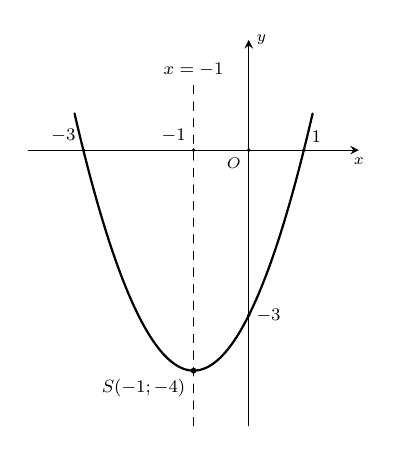
\begin{tikzpicture}[>=stealth,line join=round,line cap=round,font=\footnotesize,scale=.7]
					\def\a{1}
					\def\b{2}
					\def\c{-3}
					\draw[->] (-4,0) -- (2,0) node[below] {\scriptsize $x$};
					\draw[->] (0,-5) -- (0,2) node[right] {\scriptsize $y$};
					\draw (0,0)node[below left]{\scriptsize $O$};
					\pgfmathsetmacro\xdinh{-(\b)/2*(\a)}
					\pgfmathsetmacro\ydinh{(4*(\a)*(\c)-(\b)^2)/(4*(\a))}
					%\fill[dashed] (\xdinh,\ydinh)circle(1pt) edge (\xdinh,0) edge (0,\ydinh);
					\fill 
					(-1,0)circle(1pt)node[above left]{$-1$}
					(0,-3)circle(1pt)node[right]{$-3$}
					(-3,0)circle(1pt)node[above left]{$-3$}
					(1,0)circle(1pt)node[above right]{$1$}
					(-1,-4)circle(1.5pt)
					(0,0)circle(1pt)
					;
\draw[thick,samples=150,smooth,domain=-3.16:1.16] plot(\x,{\a*(\x)^2+(\b)*\x+(\c)})
					(-1,-4)node[below left]{$S(-1;-4)$}
					;
					\draw[dashed] (-1,-5) -- (-1,1.2)node[above]{$x=-1$};
			\end{tikzpicture}}
\item Ta có  
\allowdisplaybreaks
\begin{eqnarray*}
 && \sqrt{x^2+x+2}=5-3x \\ 
  &\Leftrightarrow& \heva{&5-3x\geq 0\\&x^2+x+2=(5-3x)^2}\\ 
  &\Leftrightarrow& \heva{&x\leq \dfrac{5}{3}\\&8x^2-31x+23=0}\\ 
  &\Leftrightarrow& \heva{&x\leq \dfrac{5}{3}\\&\hoac{&x=1\\&x=\dfrac{23}{8}}}\\ 
  &\Leftrightarrow& x=1. 
\end{eqnarray*}
Vậy nghiệm của phương trình đã cho là $x=1$.
\end{enumerate}
}
\end{bt}

\begin{bt}%[0T4B2-1]%[0T5B4-2]%[Dự án đề kiểm tra HKI NH22-23- Lương Như Quỳnh]%[Trường THPT Bắc Giang]
Cho tam giác $ABC$ có $AB=3$ cm, $AC=5$ cm và $\widehat{A}=120^\circ $.
\begin{enumerate}
\item Tính độ dài cạnh $BC$ của tam giác $ABC$.
\item Gọi $M$, $K$ lần lượt là các điểm thỏa mãn $ \overrightarrow{MB}+\overrightarrow{MC} =\overrightarrow{0}$ và $ 3\overrightarrow{KM}+\overrightarrow{KA} =\overrightarrow{0}$. Biết rằng tồn tại hai số thực $m$, $n$ để $\overrightarrow{BK}=m\overrightarrow{AB}+n\overrightarrow{AC}$. Tìm $m$, $n$.
\end{enumerate}
\loigiai{
\immini{
\begin{enumerate}
\item Áp dụng định lí Côsin ta có
\allowdisplaybreaks
\begin{eqnarray*}
 && BC^2=AB^2+AC^2-2AB\cdot AC\cdot \cos A \\ 
  &\Leftrightarrow& BC^2=3^2+5^2-2\cdot 3\cdot 5\cdot \cos 120^\circ\\ 
  &\Leftrightarrow& BC^2=49 \Rightarrow BC=7\text{ cm.} 
\end{eqnarray*}
\item Nhận xét: $M$ là trung điểm của cạnh $BC$, $K$ thuộc đoạn $AM$ sao cho $KA=3KM$.\\
Ta có $\overrightarrow{BK}=\overrightarrow{AK}-\overrightarrow{AB}=\dfrac{3}{4}\overrightarrow{AM}-\overrightarrow{AB} $.\\
Mặt khác, $M$ là trung điểm của cạnh $BC$ nên \[\overrightarrow{AM}=\dfrac{1}{2}\overrightarrow{AB}+\dfrac{1}{2}\overrightarrow{BC}.\]
\[\text{Suy ra }\overrightarrow{BK}=\overrightarrow{AK}-\overrightarrow{AB}=\dfrac{3}{4}\left(\dfrac{1}{2}\overrightarrow{AB}+\dfrac{1}{2}\overrightarrow{BC}\right)-\overrightarrow{AB} =-\dfrac{5}{8}\overrightarrow{AB}+\dfrac{3}{8}\overrightarrow{BC} .\]
Vậy $m=-\dfrac{5}{8}$, $n=\dfrac{3}{8}$.
\end{enumerate}}
{
\begin{tikzpicture}[line join= round,line cap= round, thick, font= \footnotesize, scale=.8]
			\path (0:0) coordinate (B)
			+(0:6) coordinate (C)
			+(60:3) coordinate (A)
			($(C)!1/2!(B)$) coordinate (M)
			($(A)!3/4!(M)$) coordinate (K);
			\draw (A)--(B)--(C)--cycle (A)--(M);
			\foreach \x/\g in {B/180,C/0,A/90,M/-90,K/0}
			\fill (\x) circle (1.5pt) +(\g:3mm) node{$\x$};
		\end{tikzpicture}
}
}
\end{bt}

\begin{bt}%[0T2K2-3]%[Dự án đề kiểm tra HKI NH22-23- Lương Như Quỳnh]%[Trường THPT Bắc Giang]
Một cơ sở sản xuất dự định dùng hai loại nguyên liệu để chiết xuất ít nhất $140$ kg chất A và ít nhất $9$ kg chất B. Từ mỗi tấn nguyên liệu loại I có giá $4{,}5$ triệu đồng, có thể chiết xuất được $20$ kg chất A và $0{,}6$ kg chất B. Từ mỗi tấn nguyên liệu loại II có giá $3{,}5$ triệu đồng, có thể chiết xuất được $10$ kg chất A và $1{,}5$ kg chất B. Tính chi phí ít nhất mà cơ sở sản xuất đó dự định dùng để mua nguyên liệu biết cơ sở cung cấp nguyên liệu chỉ cung cấp không quá $10$ tấn nguyên liệu loại I và không quá $9$ tấn nguyên liệu loại II.
\loigiai{
Gọi $x$, $y$ lần lượt là số nguyên liệu loại I và loại II cần dùng ($x$, $y\geq 0$).\\
Chi phí để mua nguyên liệu là $ 4x+3y $ (triệu đồng).
Theo đề bài, ta có hệ bất phương trình bậc nhất hai ẩn $x$, $y$
\[\heva{&0\leq x\leq 10\\&0\leq y\leq 9\\&20x+10y\geq 140\\&0{,}6x+1{,}5y\geq 9}\Leftrightarrow \heva{&0\leq x\leq 10\\&0\leq y\leq 9\\&2x+y\geq 14\\&2x+5y\geq 30.}\quad(*)\]
Yêu cầu bài toán trở thành: Tìm $ (x;y) $ thỏa mãn $(*)$ để $F(x;y)=4x+3y$ đạt giá trị nhỏ nhất.\\
Biểu diễn miền nghiệm của hệ $(*)$ trên mặt phẳng tọa độ $Oxy$, ta được miền tứ giác $ABCD$ (kể cả biên) với tọa độ các điểm là $A\left(\dfrac{5}{2};9\right)$, $B(10;9)$, $C(10;2)$, $D(5;4)$.\begin{center}
\begin{tikzpicture}[font=\footnotesize,line join=round, line cap=round, >=stealth,scale=0.8] 
\def \xmin{-1}\def \xmax{14}\def \ymin{-1}\def \ymax{15} 
\draw[->] (\xmin,0)--(\xmax,0) node[below left] {$x$};
\draw[->] (0,\ymin)--(0,\ymax) node[below right] {$y$};
\path (0,0) coordinate (O)
(2.5,9) coordinate (A)
(10,9) coordinate (B)
(10,2) coordinate (C)
(5,4) coordinate (D);
\foreach \x/\g in {A/90,B/45,C/45,D/-145,O/-45}
\fill (\x) circle (1.5pt) +(\g:3mm) node{$\x$};
\draw[fill=black] (0,14) circle (.5pt) node[left]{\footnotesize $14$};
\draw[fill=black] (0,9) circle (.5pt) node[above left]{\footnotesize $9$};
\draw[fill=black] (10,0) circle (.5pt) node[below right]{\footnotesize $10$};
\node at (3,12) {$2x+y=14$};
\node at (11,14) {$x=10$};
\node at (13,9.5) {$y=9$};
\node at (12,2) {$2x+5y=30$};
\begin{scope}
\clip (\xmin,\ymin) rectangle (\xmax,\ymax); 
\draw[smooth,samples=100,domain=\xmin:\xmax] plot(\x,{14-2*\x});
\draw[smooth,samples=100,domain=\xmin:\xmax] plot(\x,{6-.4*\x});
\draw[smooth,samples=100,domain=\xmin:\xmax] plot(\x,9);
\draw[smooth,samples=100] (10,\ymin)--(10,\ymax);
\fill[pattern=north east lines,opacity=.8] plot[domain=\xmin:\xmax] (\x,{6-.4*\x})--(\xmax,\ymin)--(\xmin,\ymin)--(\xmin,\ymax)--cycle;
\fill[pattern=north west lines,opacity=.8] plot[domain=\xmin:\xmax] (\x,{14-2*\x})--(\xmin,\ymin)--(\xmin,\ymax)--cycle;
\fill[pattern=north west lines,opacity=.8] (10,\ymin)--(10,\ymax)--(\xmax,\ymax)--(\xmax,\ymin)--cycle;
\fill[pattern=north east lines,opacity=.8] (\xmin,9)--(\xmin,\ymax)--(\xmax,\ymax)--(\xmax,9)--cycle;
\draw[red] (A)--(B)--(C)--(D)--cycle;
\end{scope}
\end{tikzpicture}
\end{center}
Ta có $F(A)=37$, $F(B)=67$, $F(C)=46$, $F(D)=32$.\\
Suy ra $\min F(x;y)=F(D)=32 $ đạt tại $(x;y)=(5;4)$.\\
Vậy chi phí mua nguyên liệu ít nhất là $32$ triệu đồng, khi cơ sở mua $5$ tấn nguyên liệu loại I và $4$ tấn nguyên liệu loại II.
}
\end{bt}